%----------------------------------------------------------------------------------------
%	PACKAGES AND DOCUMENT CONFIGURATIONS
%----------------------------------------------------------------------------------------

\documentclass[a4paper,11pt]{article}

\usepackage{hyperref}
\usepackage{caption}
\usepackage{xcolor}
\usepackage{graphicx} % Required for the inclusion of images
\usepackage{amsmath} % Required for some math elements 
\usepackage[margin=32mm]{geometry}
\usepackage{courier}
\usepackage{listings}

\lstset{basicstyle=\footnotesize\ttfamily,breaklines=true}
\captionsetup[figure]{font=small}

\addtolength{\topmargin}{-16mm}
\addtolength{\textheight}{32mm}


\setlength\parindent{0pt} % Removes all indentation from paragraphs
\renewcommand{\labelenumi}{\alph{enumi}.} % Make numbering in the enumerate environment by letter rather than number (e.g. section 6)


%----------------------------------------------------------------------------------------
%	DOCUMENT INFORMATION
%----------------------------------------------------------------------------------------

\title{ECEN 220 \\ Lab Report 1 \\ Signals and LTI Systems}
\author{Daniel Eisen \\ 300447549}
\date{\today}

\begin{document}
	\maketitle
	\tableofcontents
	\newpage
%----------------------------------------------------------------------------------------
%	SECTION 1
%----------------------------------------------------------------------------------------
	\section{Periodicity}
		\begin{figure}[h]
		 \begin{center}
		  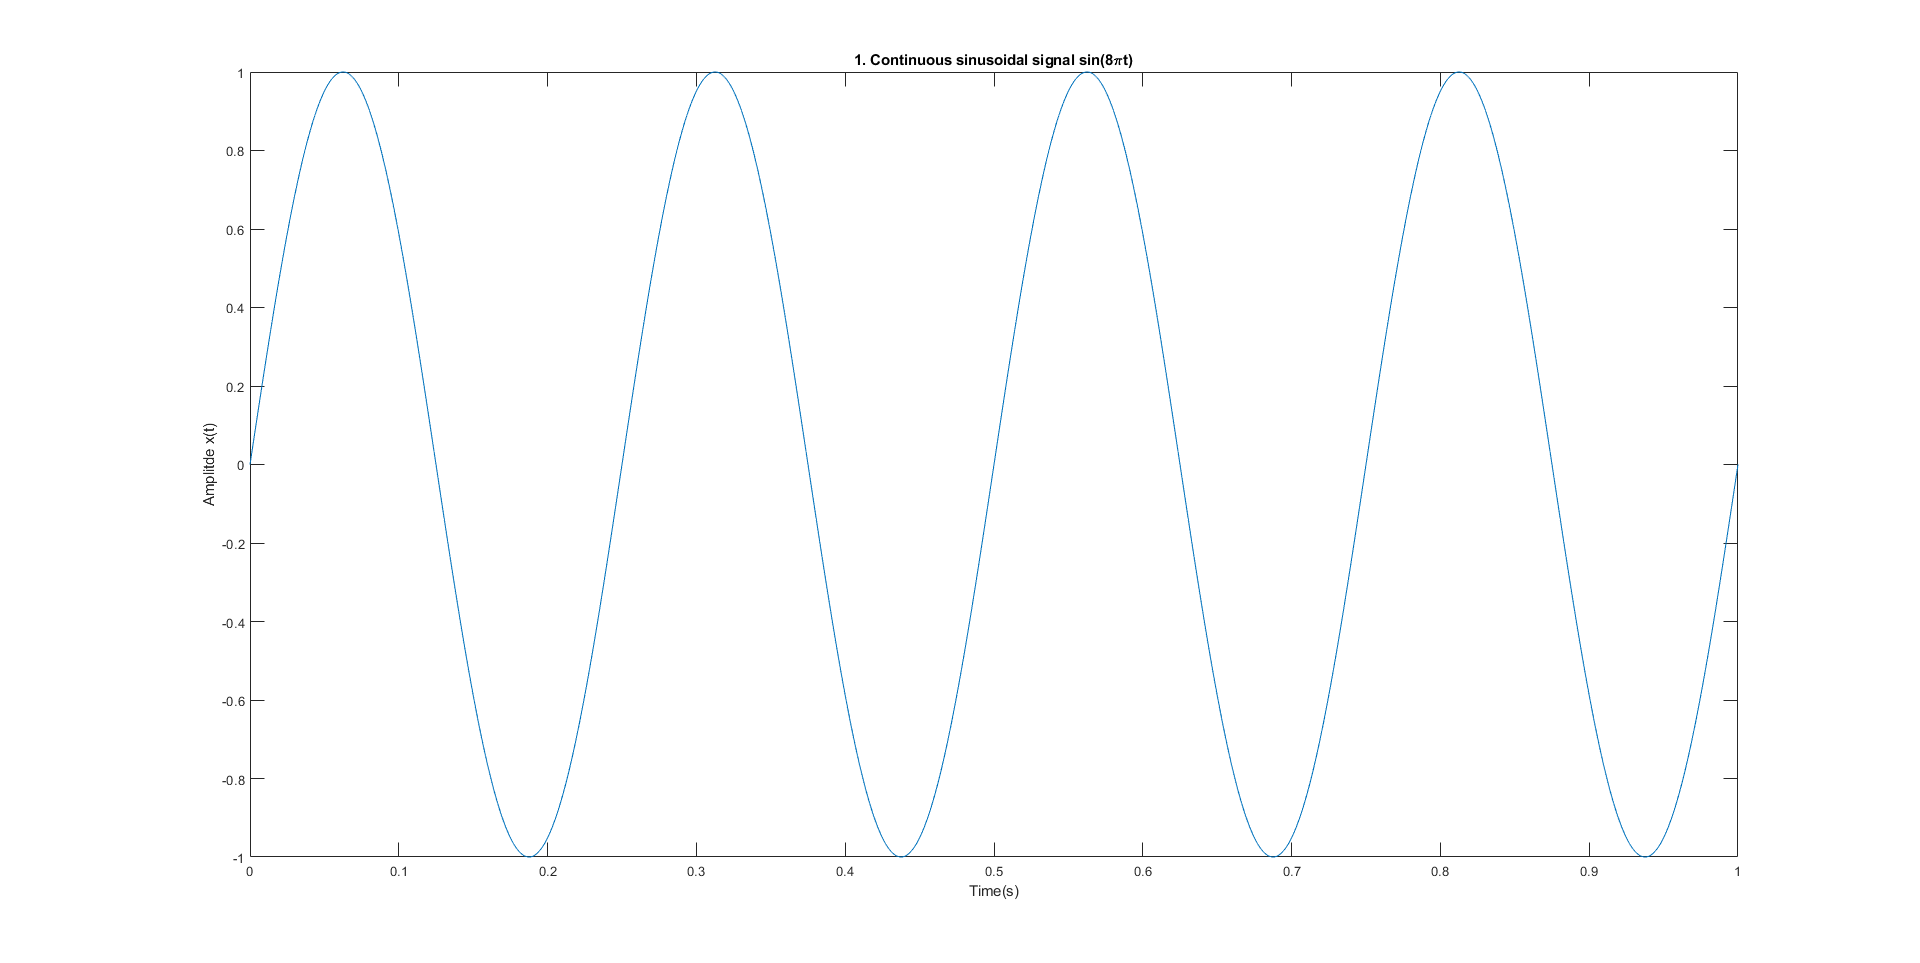
\includegraphics[width=0.7\textwidth]{1a}
		  \caption{Continuous time signal $f(x) = sin(2{\pi}f_{0}t)$}
		 \end{center}
		\end{figure}
		\subsection{Plotting Sampled Signal}
			\begin{figure}[h]
			 \begin{center}
			  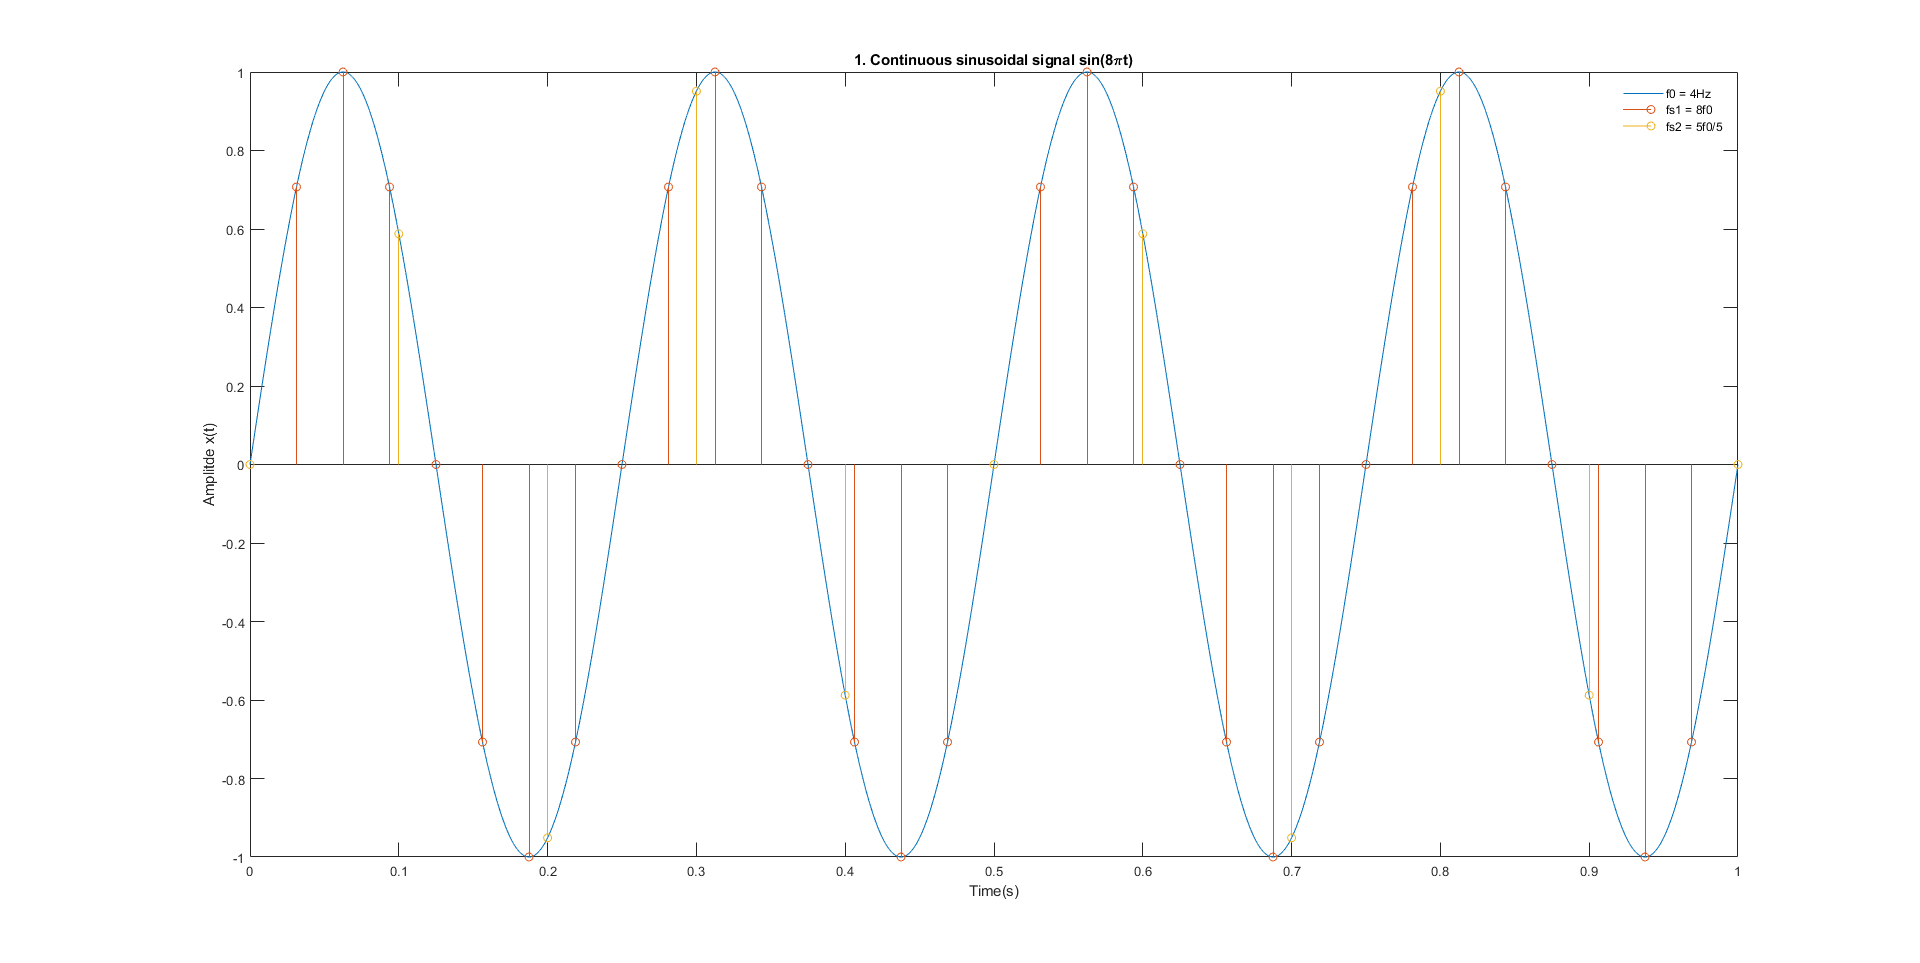
\includegraphics[width=0.65\textwidth]{1b}
			  \caption{Sampled continuous signals}
			 \end{center}
			\end{figure}
			The above shows the signal $f(x) = sin(2{\pi}f_{0}t)$ sampled in discrete time space at $8f_{0}$ and $\dfrac{5}{2}f_{0}$, ie at 32 and 10 sample respectively over a 1 second interval.
		\subsection{Discrete Periodicity Comparison}
		$$P = \dfrac{2 \pi}{\omega_{0}}$$
		The sampled signal at 32$s^{-s}$ has 8 sample per period (of CT) and thus as a period of $\dfrac{1}{4}$ ie the same as the CT signal
		The sampled signal at 10$s^{-s}$ has 4 sample per period (of CT) and thus as a period of $\dfrac{1}{2}$ ie the twice that of the CT signal
%----------------------------------------------------------------------------------------
%	SECTION 2
%----------------------------------------------------------------------------------------
\newpage
	\section{Linearity}
		\begin{figure}[h]
		 \begin{center}
		  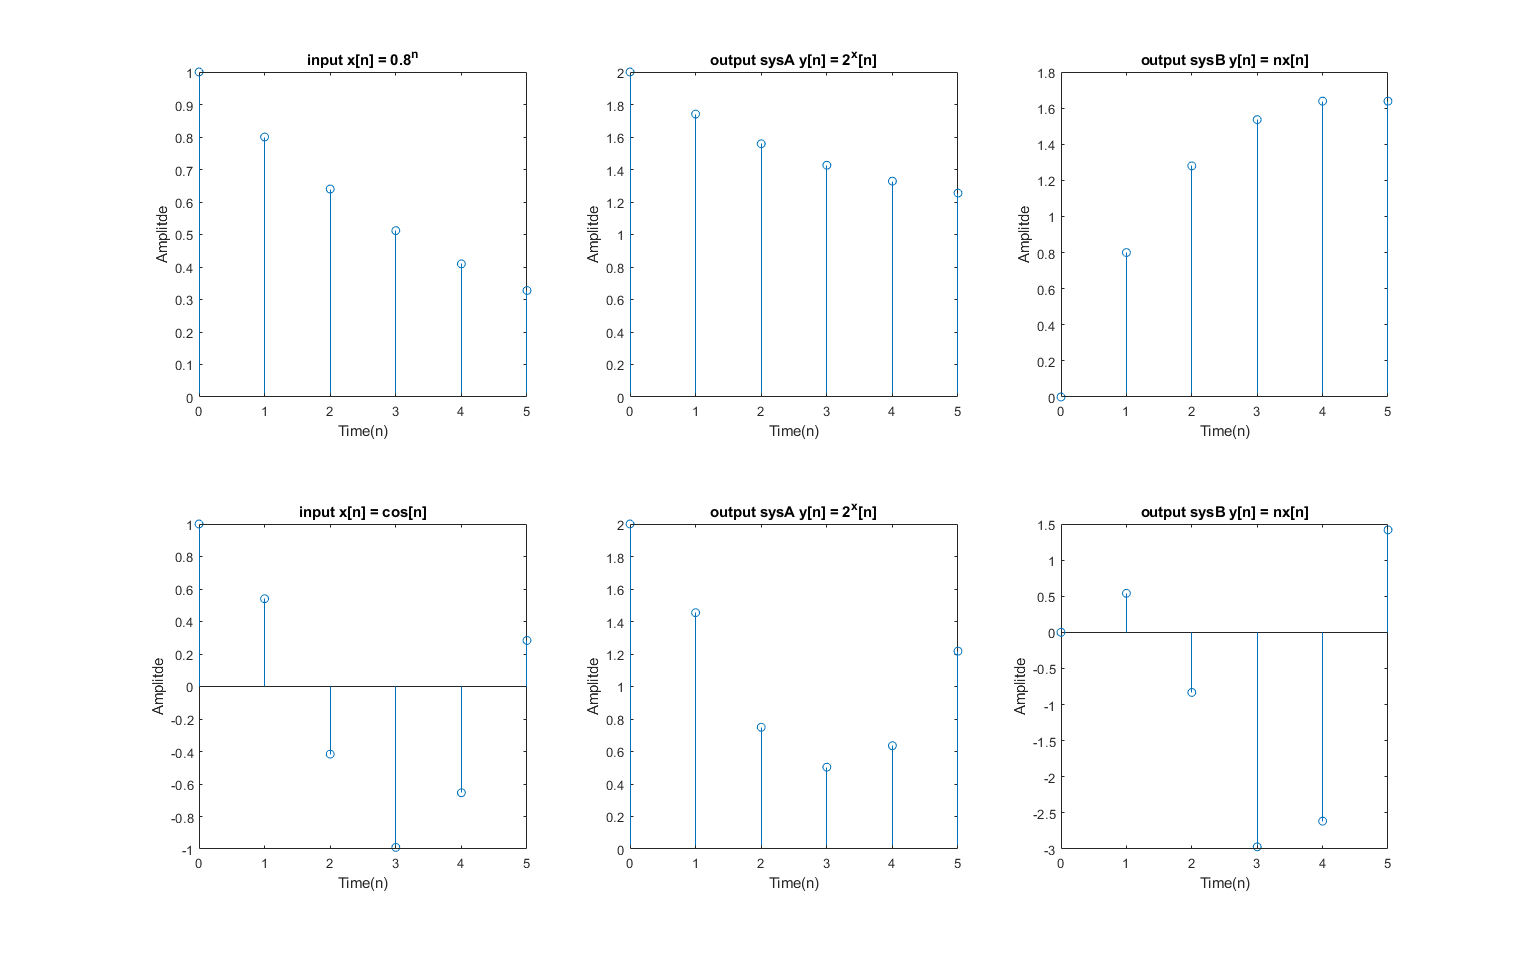
\includegraphics[width=0.65\textwidth]{2a}
		  \caption{Inputs and outputs for systems (A, B)}
		 \end{center}
		\end{figure}
		For systems A = $y[n] = 2^{x[n]}$ and B = $y[n] = nx[n]$ the above graphs plot the outputs to the respective input signals $x[n] = 0.8^{n}, cos(n)$ over the interval $0 \leq n \leq 5$
		\subsection{Test by summation}
			\begin{figure}[h]
			 \begin{center}
			  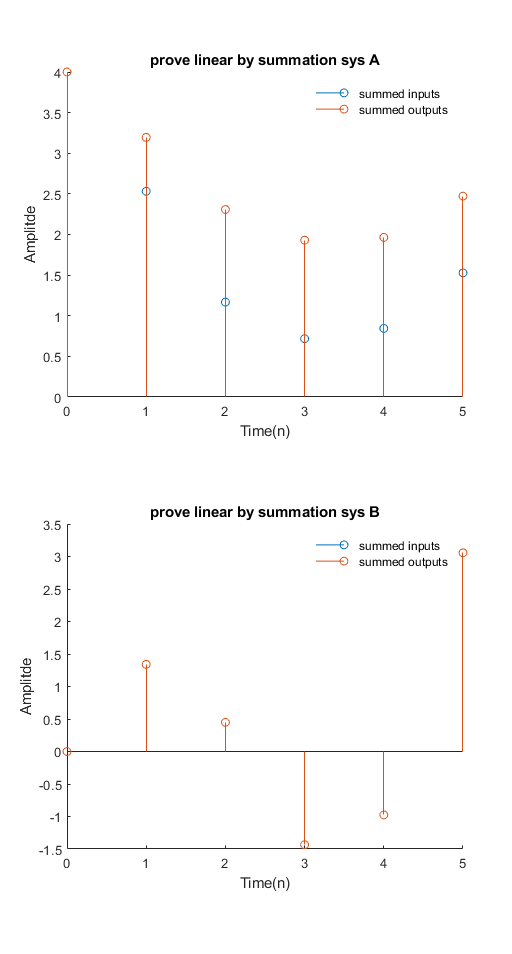
\includegraphics[width=0.25\textwidth]{2b}
			  \caption{Summed inputs vs summed outputs (A, B)}
			 \end{center}
			\end{figure}
			First test of linearity is to invoke the rule of summation. The output of the summed input signals (as an input to the system), if system is linear, should equal the summed outputs of the input signals individually.
			\begin{center}
			$y(x_{1}+x_{2}) = y(x_{1}) + y(x_{2})$
			\end{center}
			
The plot above shows this test for both systems A, and B in superposition.
This shows that System a is confirmed to be non-linear by summation and B is still a candidate for linearity by summation. 

\newpage
		\subsection{Test by scaling}
			\begin{figure}[h]
			 \begin{center}
			  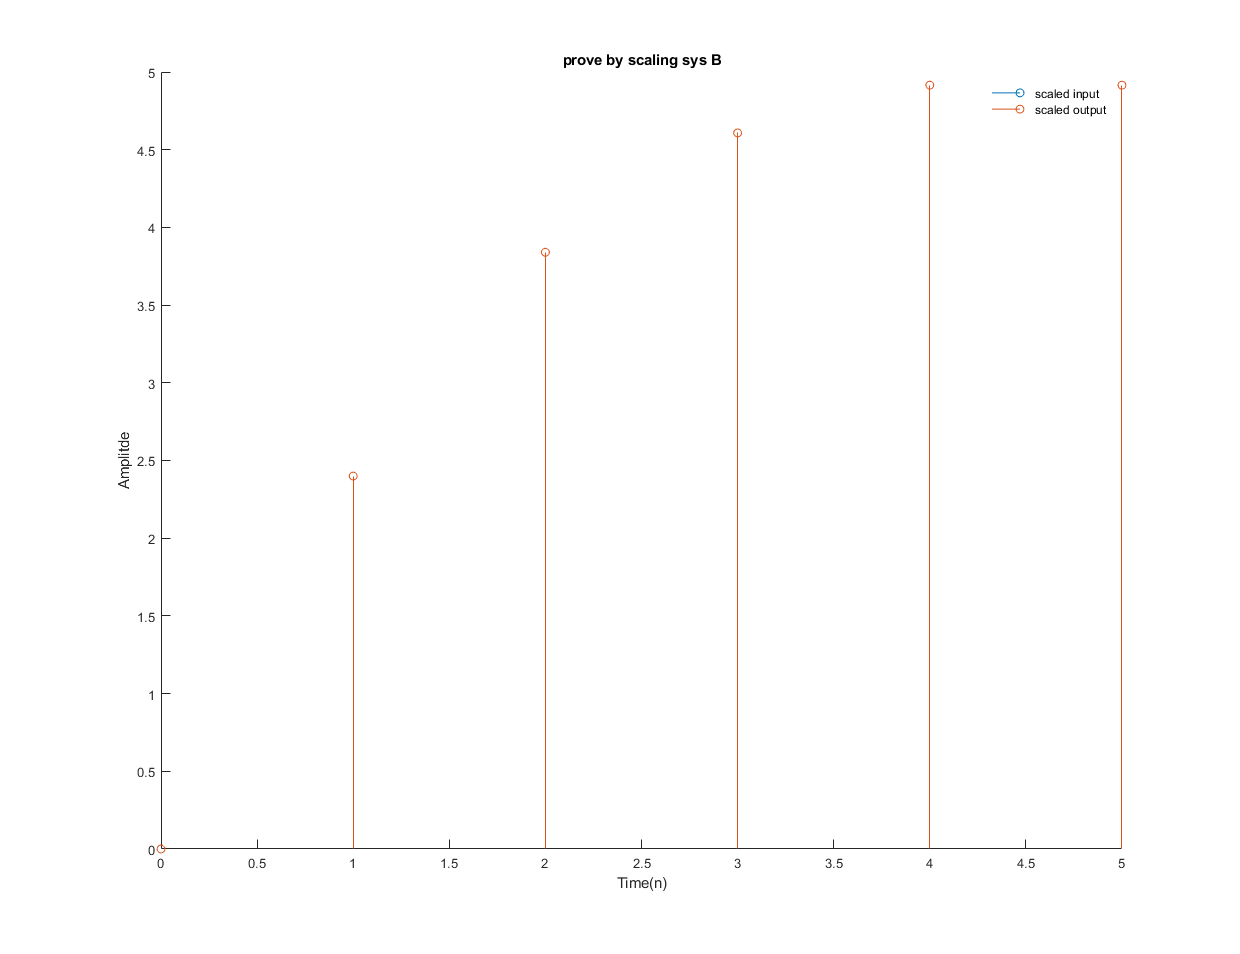
\includegraphics[width=0.5\textwidth]{2c}
			  \caption{Scaled input vs scaled output (B)}
			 \end{center}
			\end{figure}
			As B is still a candidate for linearity, the next text is that of 			scaling. The output for an input scaled be some $\alpha$ should 				equal the output (of unscaled input) scaled by the same $\alpha$.
			\begin{center}
			$\alpha y(x) = y(\alpha x)$
			\end{center}
			The plot above shows the outputs for this test (again in 						superposition) thus proving the system B's linearity.

%----------------------------------------------------------------------------------------
%	SECTION 3
%----------------------------------------------------------------------------------------
	\section{Convolution}
		\subsection{Matlab Convolution}
			\begin{figure}[h]
			 \begin{center}
			  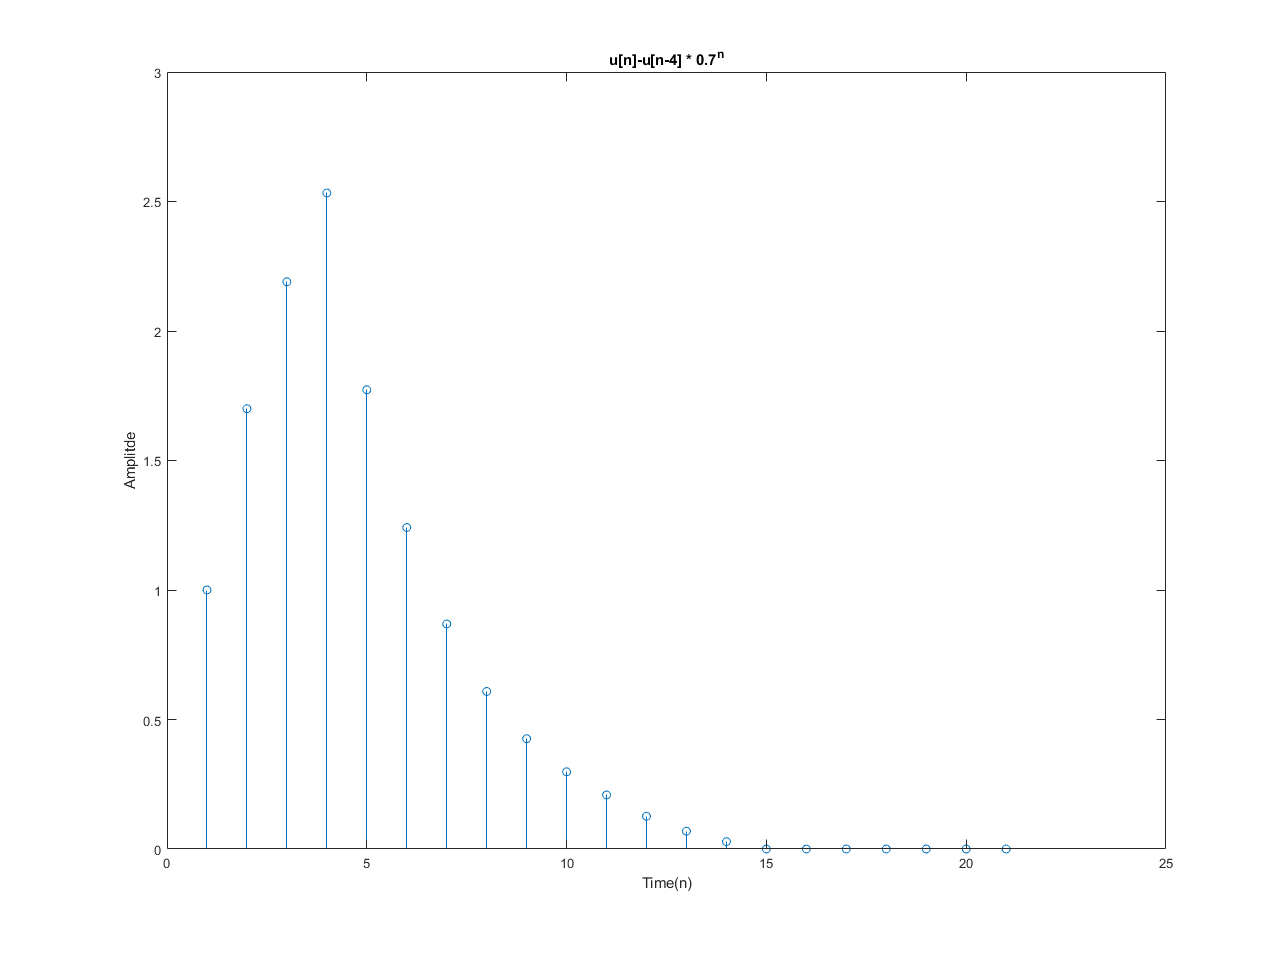
\includegraphics[width=0.65\textwidth]{3a}
			  \caption{Computational Convolution}
			 \end{center}
			\end{figure}
			The above plots the convolution of the input sequence $x[n] = u[n]-u[n-4]$ with the (DT) systems impulse response of $h[n] = 0.7^{n} : 0 \leq n \leq 10$
		
		\subsection{Manual Convolution}
			\subsubsection*{Case 1,5: No Overlap}
				$n<0, n>13 : y[n] = 0$
			\subsubsection*{Case 2: Partial Overlap Approach}
			$$0 \leq n < 3$$
			\begin{align*}
			y[n] &= \sum_{k=0}^{n} 0.7^{k} \\
			     &= \dfrac{1-0.7^{n+1}}{1-0.7} \\ \\
			y[n] &= \dfrac{1-0.7^{n+1}}{0.3} : 0 \leq n < 3
			\end{align*}
			
			\subsubsection*{Case 2: Complete Overlap}
			$$n \leq 10, n-3 \geq 0 \Rightarrow 0 \leq n \leq 10$$			
			\begin{align*}
			y[n] &= \sum_{k=n-3}^{n} 0.7^{k} \\
			     &= \sum_{k=0}^{n} 0.7^{k} - \sum_{k=0}^{n-4} 0.7^{k} \\
			     &= \dfrac{1-0.7^{n+1}}{0.3} - \dfrac{1-0.7^{n-3}}{0.3} \\ \\
			y[n] &= \dfrac{0.7^{n-3}-0.7^{n+1}}{0.3} : 3 \leq n \leq 10		
			\end{align*}
			\subsubsection*{Case 2: Partial Overlap Departure}
			$$n > 10, n-3 \leq 10 \Rightarrow 10 < n \leq 13$$			
			\begin{align*}
			y[n] &= \sum_{k=n-3}^{10} 0.7^{k} \\
			     &= \sum_{k=0}^{10} 0.7^{k} - \sum_{k=0}^{n-4} 0.7^{k} \\
			     &= \dfrac{1-0.7^{11}}{0.3} - \dfrac{1-0.7^{n-3}}{0.3} \\ \\
			y[n] &= \dfrac{0.7^{n-3}-0.7^{11}}{0.3} : 10 < n \leq 13		
			\end{align*}
			\subsubsection*{Piecewise Defined}
			\[ y[n]=\begin{cases}
				0 & n<0 \\ \\
      			\dfrac{1-0.7^{n+1}}{0.3} &  0 \leq n < 3 \\ \\
      			\dfrac{0.7^{n-3}-0.7^{n+1}}{0.3} & 3 \leq n \leq 10 \\ \\
      			\dfrac{0.7^{n-3}-0.7^{11}}{0.3} & 10 < n \leq 13 \\ \\
      			0 & n>13
   				\end{cases}
			\]

%----------------------------------------------------------------------------------------
%	APPENDIX
%----------------------------------------------------------------------------------------
\newpage
\section{Appendix}

\subsection*{Figure 1, 2:}
\addcontentsline{toc}{subsection}{Figure 1, 2}
\lstinputlisting{q1.m}

\subsection*{Figure 3:}
\addcontentsline{toc}{subsection}{Figure 3}
\lstinputlisting{q2a.m}

\subsection*{Figure 4:} 
\addcontentsline{toc}{subsection}{Figure 4}
\lstinputlisting{q2b.m}
\newpage
\subsection*{Figure 5:}
\addcontentsline{toc}{subsection}{Figure 5}
\lstinputlisting{q2c.m}

\subsection*{Figure 6:}
\addcontentsline{toc}{subsection}{Figure 6} 
\lstinputlisting{q3a.m}

\end{document}
